\documentclass[10pt]{beamer}

\usetheme[numbering=fraction]{metropolis}
\usepackage{appendixnumberbeamer}
\setbeamercovered{transparent}
\usepackage{xcolor,colortbl}

\usepackage{amsmath,amssymb,booktabs}
\usepackage[scale=2]{ccicons}
\usepackage[round]{natbib}
\usepackage{pgfplots}
\usepgfplotslibrary{dateplot}
\usepackage{graphicx}
\graphicspath{{./}}
\usepackage{etoolbox} 
\usepackage{caption} 

\newcommand{\themename}{\textbf{\textsc{metropolis}}\xspace}
\setbeamertemplate{frame footer}{Pisharam\hfill Peer-Effects in ESB Adoption \hfill Spring 2025}
\setbeamerfont{page number in head/foot}{size=\tiny}
\setbeamercolor{footline}{fg=white, bg=mDarkTeal}

\title{Peer-Effects in Electric School Bus Adoption}
\subtitle{Brown Bag: Applied Microeconomics (Spring 2025)}
\author{Anirudh Pisharam}
\institute{Department of Economics}
\date{\today}

\AtBeginSection[]
{
  \begin{frame}{Outline}
    \tableofcontents[currentsection]
  \end{frame}
}

\begin{document}

\maketitle

\begin{frame}{Outline}
  \tableofcontents
\end{frame}

%======================================================================
\section{Motivation \& Setting}
%======================================================================

\begin{frame}{Why Electric School Buses (ESBs) provide a unique setting?}

  \begin{itemize}
    \item \textbf{High Cost:} \$300k ESB vs \$100k diesel
    \item \textbf{High Uncertainty:} Range anxiety, charging logistics, cold weather performance
    \item \textbf{Policy Scale:} \alert{\$5 Billion} announced federal funding (EPA Clean School Bus Program)
    \item Interesting setting for $\textbf{peer-effects}$ (and potentially \alert{social learning}) in the public sector
  \end{itemize}
\end{frame}

\begin{frame}[label=core_question]{The Core Question: Contagion or Coincidence?}
  \frametitle{The Core Question: Contagion or Coincidence?}
  \framesubtitle{Disentangling Peer Influence from Shared Characteristics}

  \begin{itemize}
    \item We observe strong spatial clustering of adoptions
    \item \textbf{Is it Contagion?} Does a neighbor's choice \textit{cause} my choice (Peer Effects)?
    \item \textbf{Or is it Coincidence?} Do neighbors simply share the same climate, politics, and state policies (Correlated Shocks)?
  \end{itemize}
  
  \vspace{1em}
  \hyperlink{backup_own_adoption}{\textbf{\color{mLightBrown} $\rightarrow$ See Determinants of Own Adoption}}
\end{frame}

\begin{frame}{Early Trends: Participation Map}
  \frametitle{Early Trends: Participation Map}
  \framesubtitle{Federally-funded ESB awards (2022-2023)}

  \begin{figure}
    \centering
    \begin{figure}
        \centering
        
\includegraphics[width=0.9\textwidth]{Social Learning/Applied Micro BB (Fall 2025)/esb_adoption_by_year_map.png}
        \caption{Map of Electric School Bus \textbf{awards} in the Continental US }
        \label{fig:placeholder}
    \end{figure}    
  \end{figure}
\end{frame}

\begin{frame}{Two Potential Channels (The Mechanisms)}
  \frametitle{Two Potential Channels (The Mechanisms)}
  \framesubtitle{What do we mean by "peer effects"?}

  \begin{columns}[T]
    \begin{column}{0.5\textwidth}
      \textbf{1. Emulation (Reputation)}
      \begin{itemize}
        \item "Keeping up with the Joneses"
        \item Mechanism: \alert{Visibility} \& Rivalry
        \item Likely \alert{non-negative}
      \end{itemize}
    \end{column}
    \begin{column}{0.5\textwidth}
      \textbf{2. Information from Non-Local Peers (Regional Ring)}
      \begin{itemize}
        \item Reducing technical uncertainty
        \item Mechanism: \alert{Similar operating conditions} beyond immediate neighbors
        \item Can be \alert{positive} (success) or \alert{negative} (discouragement)
      \end{itemize}
    \end{column}
  \end{columns}
\end{frame}

%======================================================================
\section{Identification Strategy: The "How"}
%======================================================================

\begin{frame}{The Identification Challenge}
  \textbf{The Manski (1993) Reflection Problem}
  \begin{equation*}
    Y_i = \underbrace{\beta (W Y)_i}_{\text{Endogenous}} + \underbrace{\gamma X_i + \delta (W X)_i}_{\text{Contextual}} + \underbrace{\alpha_i + \epsilon_i}_{\text{Correlated}}
  \end{equation*}

  \begin{itemize}
    \item We see A and B adopt. Did A copy B, or did a state subsidy hit both?
    \item \alert{Solution:} We need an exogenous shock that moves Peers ($Y_j$) but not Focal District ($Y_i$)
  \end{itemize}
\end{frame}

\begin{frame}{Our Solution: The EPA Lottery}
  \frametitle{Our Solution: The EPA Lottery}
  \framesubtitle{A Gold-Standard Instrument}

  \begin{itemize}
    \item \textbf{The Program:} EPA Clean School Bus Program (Rounds 1 \& 3)
    \item \textbf{The Mechanism:} Oversubscribed funding allocated via \textbf{LOTTERY}
    \item \textbf{The Data Win:} We obtained the list of \alert{Waitlisted Applicants}
    \item \textbf{Randomization:} As-good-as random \textbf{within priority strata}; we condition on \texttt{is\_priority}.
  \end{itemize}

  \vspace{1em}
  \textbf{The Instrument ($Z$):}
  For the applicant pool, a peer's lottery win is \alert{randomly assigned}.
  $$ Z_{j} = \mathbb{I}(\text{Peer } j \text{ won lottery}) $$
\end{frame}

\begin{frame}[label=validating_design]{Validating the Design: The "Strata" Fix}
  \frametitle{Validating the Design: The "Strata" Fix}
  \framesubtitle{Addressing Selection Bias}

  \begin{columns}[T]
    \begin{column}{0.5\textwidth}
      \textbf{Problem: Naive Balance Masks Bias}
      \begin{itemize}
        \item Aggregated data looks balanced on income ($p>0.50$).
        \item \textbf{BUT:} Stratified tests reveal selection bias in the "Non-Priority" pool.
      \end{itemize}
    \end{column}
    \begin{column}{0.5\textwidth}
      \textbf{Solution: Stratified Balance}
      \begin{itemize}
        \item Within "Priority" buckets, the lottery is cleaner.
        \item Control for \texttt{is\_priority} and demographics.
      \end{itemize}
    \end{column}
  \end{columns}
  
  \vspace{1em}
  \centering
  \alert{Identification relies on: $Z \perp \epsilon \mid \text{Priority Status and other observables}$}
  
  \vspace{1em}
  \hyperlink{backup_balance}{\textbf{\color{mLightBrown} $\rightarrow$ See Balance Tables}}
\end{frame}

\begin{frame}{Separating Channels: Spatial Matrices}
To disentangle mechanisms, we estimate the following 2SLS model:
\small
\[
\text{Adopt}_i
= \beta_E\,\widehat{(W_{geo}\, \text{Adopt})}
+ \beta_R\,\widehat{(W_{clim}\, \text{Adopt})}
+ \gamma X_i + \varepsilon_i
\]

\begin{itemize}\setlength\itemsep{0.25em}
  \item \textbf{Emulation ($W_{geo}$):} KNN-6 nearest districts — visibility/rivalry.
  \item \textbf{Regional ring ($W_{clim}$):} KNN-20 \emph{minus} KNN-6 (neighbors 7–20) — info from non-local, similar conditions. \emph{Currently distance-based; climate-similarity $W$ planned.}
  \item Charter Schools currently filtered out
\end{itemize}

\medskip
\hyperlink{backup_spatial}{\textbf{\color{mLightBrown}Spatial Construction Details}}
\hspace{0.8em}| \hspace{0.8em}
\hyperlink{backup_lea_waterfall}{\textbf{\color{mLightBrown}Sample Filtering Waterfall}}
\end{frame}


%======================================================================
\section{Results}
%======================================================================

\begin{frame}[label=main_results]{Main Results: Naive OLS vs. Causal 2SLS}
  \begin{table}
    \centering
    \small
    \begin{tabular}{l c c}
      \toprule
       & \textbf{(1) Naive OLS} & \textbf{(2) 2SLS (IV)} \\
      \midrule
      \textbf{Peer Effects} & & \\
      Emulation ($\mathbf{W}_{geo} \cdot Y$) & 0.115*** & \textbf{0.053} \\
       & (0.019) & (0.039) \\
      Regional Ring ($\mathbf{W}_{clim} \cdot Y$) & 0.161*** & \textbf{0.152***} \\
       & (0.027) & (0.045) \\
      \midrule
      \textbf{Controls} & & \\
      Priority Status & 0.106*** & 0.108*** \\
      Log(Income) & -0.020** & -0.021** \\
      \midrule
      \textit{SW Partial F (Geo)} & -- & \textbf{11,955} \\
      \textit{SW Partial F (Ring)} & -- & \textbf{5,292} \\
      \bottomrule
    \end{tabular}
  \end{table}

  \vspace{-0.5em}
  \textbf{Interpretation:} Instrumented estimates indicate a \textbf{causal equilibrium peer spillover} from non-local peers (regional ring); the local emulation coefficient attenuates once instrumented. Mechanism (learning vs other) left for follow-up tests.

  \vspace{0.4em}
  {\footnotesize \textit{Spec:} Outcome = \texttt{IS\_ADOPTER}; Endog = \{$\mathbf{W}_{geo}Y$, $\mathbf{W}_{clim}Y$\}; IVs = \{$\mathbf{W}_{geo}Z$, $\mathbf{W}_{clim}Z$\}; FE = state; SE = state-clustered; Sample = matched traditional districts.}

  \vspace{0.5em}
  \hyperlink{backup_peer_effects}{\textbf{\color{mLightBrown} $\rightarrow$ See Full Estimates (incl. Own Lottery Win as sensitivity)}}
\end{frame}

%======================================================================
\section{Discussion \& Next Steps}
%======================================================================

\begin{frame}{Implications \& Mechanism Roadmap}
  \textbf{1. Policy Implication}
  \begin{itemize}
    \item Priority status strongly predicts adoption (consistent with program rules)
    \item Peer spillovers appear economically meaningful
  \end{itemize}

  \vspace{1em}
  \textbf{2. Threat 2: Measurement of "Outcome"}
  \begin{itemize}
      \item \textbf{Problem:} To test learning, we need to know if a peer had a "Good" or "Bad" experience
      \item \textbf{Data 1 (Gold):} Survey data (currently small sample)
      \item \textbf{Data 2 (Silver):} Local news sentiment analysis (factiva/NexisUni)
      \item \textbf{Data 3 (Bronze):} Revealed Preference (Does the peer apply again in Round 3?)
  \end{itemize}
  
  \vspace{1em}
  \alert{Next Step:} Interact $\widehat{PeerAdopt}$ with peer's \textit{Outcome Quality} to identify discouragement.
\end{frame}

\begin{frame}{Feedback \& Next Steps}
\begin{columns}[T]
\begin{column}{0.5\textwidth}
\textbf{Feedback Requested}
\begin{itemize}
  \item \textbf{Peer network/definition:} Keep KNN-6 (local) + “regional ring”; add a climate-similarity $W$; consider dealer/utility and border-pair links.
  \item \textbf{Exclusion threats:} Could neighbor wins affect me via dealer/utility capacity or state targeting (non-info channels)?
  \item \textbf{Discouragement:} Good pointers to negative social learning papers?
\end{itemize}
\end{column}
\begin{column}{0.5\textwidth}
\textbf{Next Steps}
\begin{itemize}
  \item \textbf{Lags/event-time:} Neighbor win/delivery at $t\!-\!1 \rightarrow$ own apply/adopt at $t$.
  \item \textbf{Fixed effects:} Year FE + state$\times$year; (later) utility/dealer-region$\times$year.
  \item \textbf{Network build:} Implement climate-$W$; keep leave-one-out weights; run border-donut robustness.
  \item \textbf{Robustness:} Logit/probit with control-function for binary Y; compare marginal effects to 2SLS-LPM.
\end{itemize}
\end{column}
\end{columns}
\end{frame}


%======================================================================
\appendix
% Reset frame counter for appendix
\setcounter{framenumber}{0}
\setbeamertemplate{frame numbering}{%
  A\insertframenumber%
}
\section{Appendix}
%======================================================================

\begin{frame}[label=backup_own_adoption]{Backup: Determinants of Own Adoption (OLS)}
  \centering
  \scriptsize
  \begin{tabular}{l c c c}
    \toprule
    & \textbf{Model 1} & \textbf{Model 2} & \textbf{Model 3} \\
    & (Naive) & (With Priority) & (Interaction) \\
    \midrule
    Log(Median Income) & -0.022** & -0.011 & -0.012 \\
    Poverty Rate & 0.177*** & 0.138*** & 0.132 \\
    Log(Enrollment) & 0.026*** & 0.025*** & 0.025*** \\
    \% Hispanic & -0.019 & -0.024 & -0.024 \\
    Priority Status & -- & \textbf{0.110***} & 0.101*** \\
    Priority $\times$ Poverty & -- & -- & 0.061 (ns) \\
    \bottomrule
  \end{tabular}
  
  \vspace{1em}
  \textbf{Key:} Income effect disappears when controlling for Priority Status. EPA rules drive the income correlation.
  \vspace{1em}
  
  \hyperlink{core_question}{\beamerreturnbutton{Return to Main Presentation}}
\end{frame}

\begin{frame}[label=backup_balance]{Backup: Balance Table (The "Strata" Proof)}
  \centering
  \tiny
  \begin{tabular}{l c c c c}
    \toprule
    \textbf{Variable} & \textbf{Mean (Winners)} & \textbf{Mean (Losers)} & \textbf{Diff} & \textbf{P-Val} \\
    \midrule
    \multicolumn{5}{l}{\textbf{Panel A: Naive (All Applicants)}} \\
    Median Income & 65,164 & 65,863 & -698 & 0.534 \\
    Poverty Rate & 0.14 & 0.14 & 0.00 & 0.511 \\
    \% Hispanic & 0.11 & 0.13 & -0.02 & \textbf{0.004***} \\
    \midrule
    \multicolumn{5}{l}{\textbf{Panel B: Priority Applicants Only (N=1,220)}} \\
    Median Income & 54,050 & 55,002 & -952 & 0.425 \\
    Poverty Rate & 0.17 & 0.16 & 0.00 & 0.432 \\
    Enrollment & 10,076 & 6,193 & 3,883 & \textbf{0.049**} \\
    \midrule
    \multicolumn{5}{l}{\textbf{Panel C: Non-Priority Applicants Only (N=1,332)}} \\
    Median Income & 68,050 & 81,142 & -13,091 & \textbf{0.000***} \\
    Poverty Rate & 0.13 & 0.10 & 0.03 & \textbf{0.000***} \\
    \bottomrule
  \end{tabular}
  
  \vspace{1em}
  \normalsize
  \textbf{Takeaway:} Naive balance masks heterogeneity. Priority/Non-Priority groups are distinct. 
  \vspace{1em}
  
  \hyperlink{validating_design}{\beamerreturnbutton{Return to Main Presentation}}
\end{frame}

% --- Backup: Sample filtering waterfall ---
\begin{frame}[label=backup_lea_waterfall]{Backup: Sample Filtering (LEA Types)}
\centering
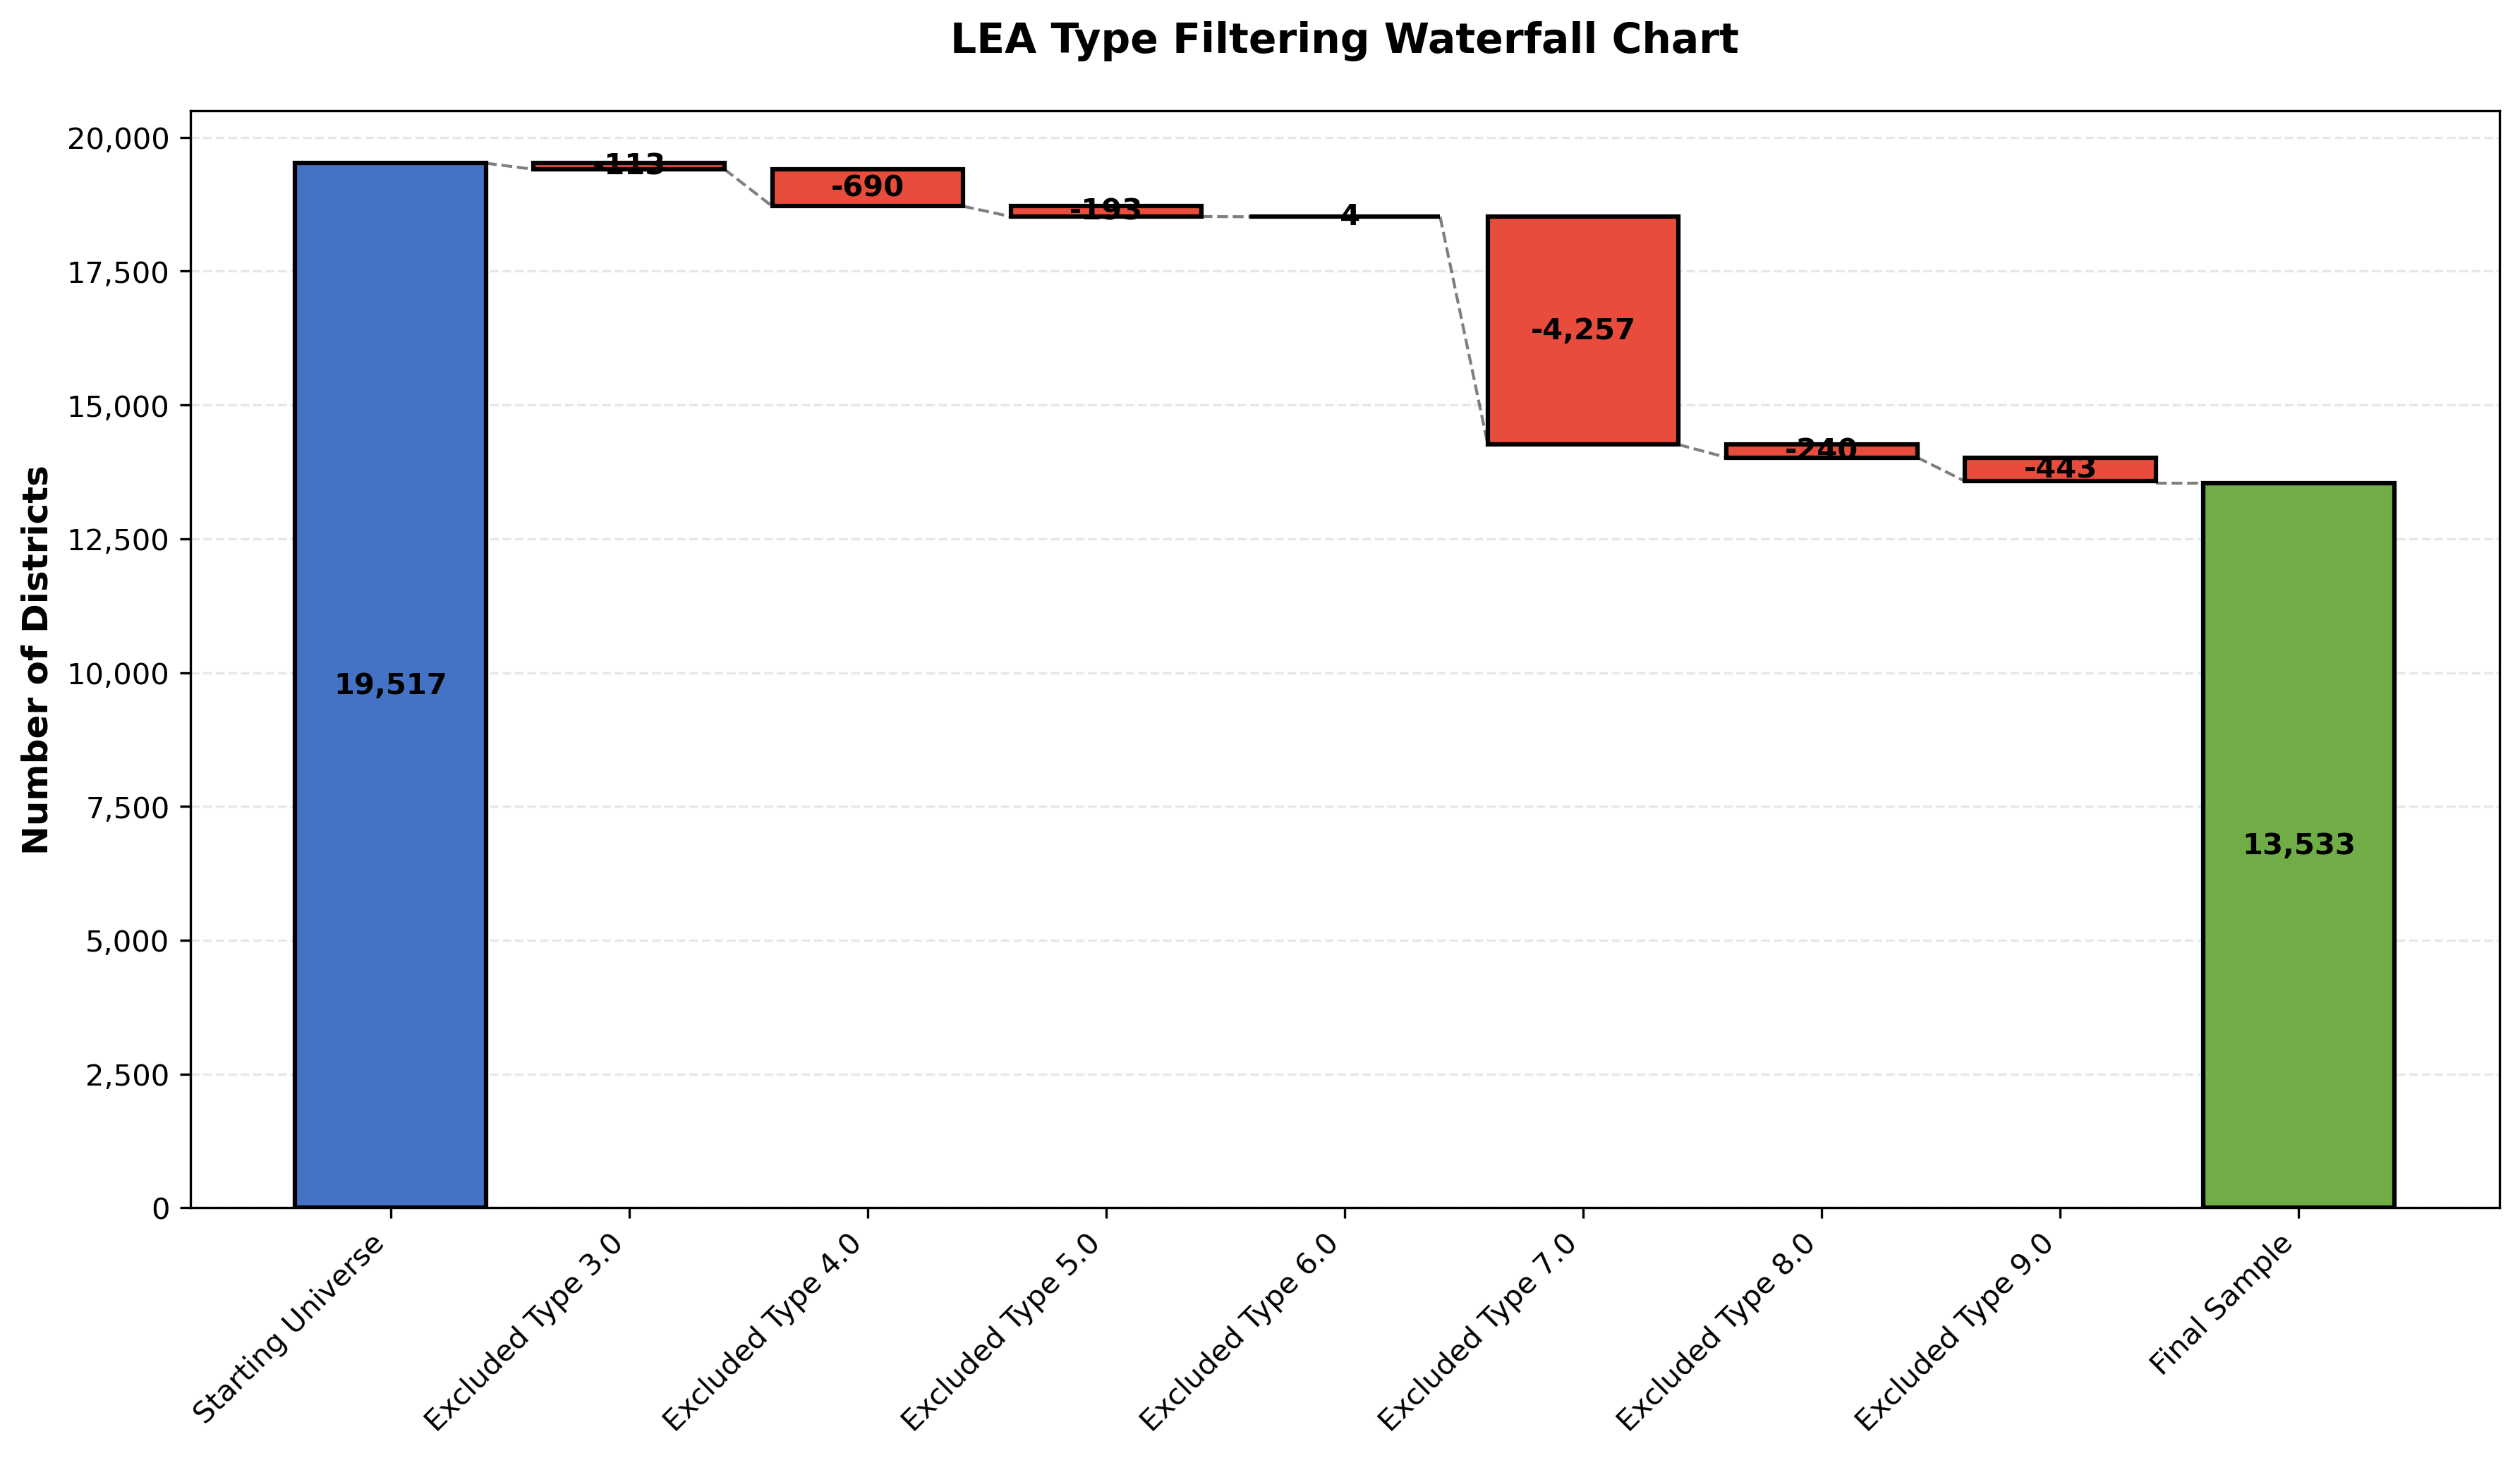
\includegraphics[width=\textwidth]{lea_type_filtering_waterfall.png}

\vspace{0.3em}
\scriptsize
Notes: Starting universe = 19{,}517 districts; final analysis sample = 13{,}533 after excluding LEA types 3, 4, 5, 6, 7, 8, 9.
\par
\hyperlink{core_question}{\beamerreturnbutton{Return to Main}}
\end{frame}


\begin{frame}[label=backup_spatial]{Backup: Spatial Matrix Construction}
    \textbf{1. Emulation Matrix ($\mathbf{W}_{geo}$)}
    \begin{itemize}
        \item Calculated using K-Nearest Neighbors with $k=6$.
        \item Captures the closest 6 districts (centroids).
    \end{itemize}
    
    \vspace{1em}
    \textbf{2. Regional Ring Matrix ($\mathbf{W}_{clim}$)}
    \begin{itemize}
        \item Calculated using K-Nearest Neighbors with $k=20$.
        \item \textbf{Orthogonalization:} We subtract the set of neighbors in $\mathbf{W}_{geo}$ from this set.
        \item \textit{Result:} A "donut" of neighbors 7 through 20.
        \item Ensures that $\beta_E$ and $\beta_R$ are identified from \textbf{distinct} sets of peers.
        \item \emph{Planned robustness:} Replace with a \textbf{climate-similarity} matrix (HDD/CDD/winter lows) to test mechanism.
    \end{itemize}
    
    \vspace{1em}
    \hyperlink{main_results}{\beamerreturnbutton{Return to Main Presentation}}
\end{frame}


\begin{frame}[label=backup_peer_effects]{Backup: Peer Effects Estimates (Full)}
  \centering
  \scriptsize
  \begin{tabular}{l c c c}
    \toprule
    & \textbf{(1) Naive OLS} & \textbf{(2) 2SLS (A)} & \textbf{(3) 2SLS (B)} \\
    \midrule
    \textbf{Peer Effects} & & & \\
    Emulation ($\mathbf{W}_{geo}$) & 0.115*** & 0.053 & 0.041** \\
    Regional Ring ($\mathbf{W}_{clim}$) & 0.161*** & 0.152*** & -0.025 \\
    \midrule
    \textbf{Select Controls} & & & \\
    Priority Status & 0.106*** & 0.108*** & 0.052*** \\
    Own Lottery Win (IV\_Z) & -- & -- & 0.962*** \\
    \midrule
    First Stage F (Geo) & -- & 11,955 & 11,564 \\
    First Stage F (Ring) & -- & 5,292 & 5,173 \\
    R-Squared & 0.072 & 0.071 & 0.779 \\
    \bottomrule
  \end{tabular}
  
  \vspace{1em}
  \normalsize
  \textbf{Discussion:} Model (3) includes \texttt{Own Lottery Win} in the outcome—\textit{not preferred} for peer-effects identification; shown only as a sensitivity. Main specification is Model (2) with instruments \{$\mathbf{W}_{geo}Z$, $\mathbf{W}_{clim}Z$\} and no own-$Z$ control.
  
  \vspace{0.5em}
  \hyperlink{main_results}{\beamerreturnbutton{Return to Main Presentation}}
\end{frame}

\end{document}
